\chapter{How does a computer work?}
\epigraph{The good news about computers is that they do what you tell them to do. The bad news is that they do what you tell them to do.}{Ted Nelson}

In the general public, it is well known that computers effectively know only two states -- current flows or does not. These \emph{bits} of information are commonly represented by the digits 1 and 0. But how can these elementary states be assembled into complex programs?

\section{Binary Representation of Numbers}
Before we get to understand how, internally, \emph{programs} look like, let us first have a look at \emph{numbers}, ...

\subsection{Binary Representation of Positive Integers} \label{sec:BinaryNumbers}
... and more simply, positive integers. For that, let us start in the familiar decimal system, and look at a random number, say $1725$:
%
\begin{defbox}[Decomposition of a decimal integer]
\begin{center}
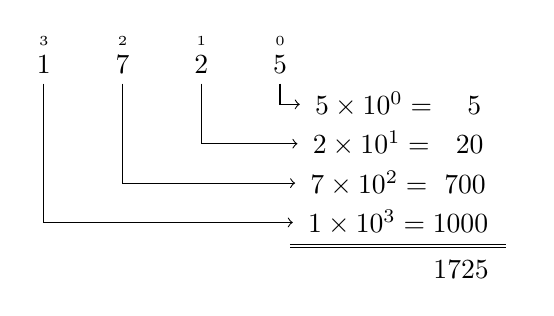
\begin{tikzpicture}[
  flow/.style={draw=black,->,shorten >=2pt}
]
  \node (s3) at (0, 2.3) {\tiny 3};
  \node (s2) at (1, 2.3) {\tiny 2};
  \node (s1) at (2, 2.3) {\tiny 1};
  \node (s0) at (3, 2.3) {\tiny 0};

  \node (n3) at (0, 2) {1};
  \node (n2) at (1, 2) {7};
  \node (n1) at (2, 2) {2};
  \node (n0) at (3, 2) {5};

  \node (e3) at (4.5, 0.0) {$1 \times 10^3 = 1000$};
  \node (e2) at (4.5, 0.5) {$7 \times 10^2 = ~700$};
  \node (e1) at (4.5, 1.0) {$2 \times 10^1 = ~~20$};
  \node (e0) at (4.5, 1.5) {$5 \times 10^0 = ~~~5$};

  \draw[flow] (n3.south) |- (e3.west);
  \draw[flow] (n2.south) |- (e2.west);
  \draw[flow] (n1.south) |- (e1.west);
  \draw[flow] (n0.south) |- (e0.west);
  
  \node (l0) at (3.0, -0.3) {};
  \node (l1) at (6.0, -0.3) {};
  \draw[double] (l0) -- (l1);
  
  \node (re) at (5.3, -0.6) {$1725$};
\end{tikzpicture}
\end{center}
\end{defbox}

We start by enumerating the digits of our number $1725$ \emph{from the right} and \emph{starting with $0$}; indices will be called \emph{exponents}, and the reason for that will become clear in a second. The contribution of each digit to the whole number ist given by the product of the digit's value and the power of base $10$ to the exponent. Summing up all individual contributions restores the number from which we started -- $1725$.

This may seem a tedious and very technical exercise in a concept we've known since primary school. The benefit of these considerations is the realization that the same concept can be applied to other \emph{base systems} as well: if we don't have ten digits (as in our \emph{decimal system}), but only two (\ie if we use the \emph{binary system}), then all we have to do is to replace the base $10$ with base $2$ and follow the same rules. For example, we find:

\begin{defbox}[Decomposition of a binary integer]
\begin{center}
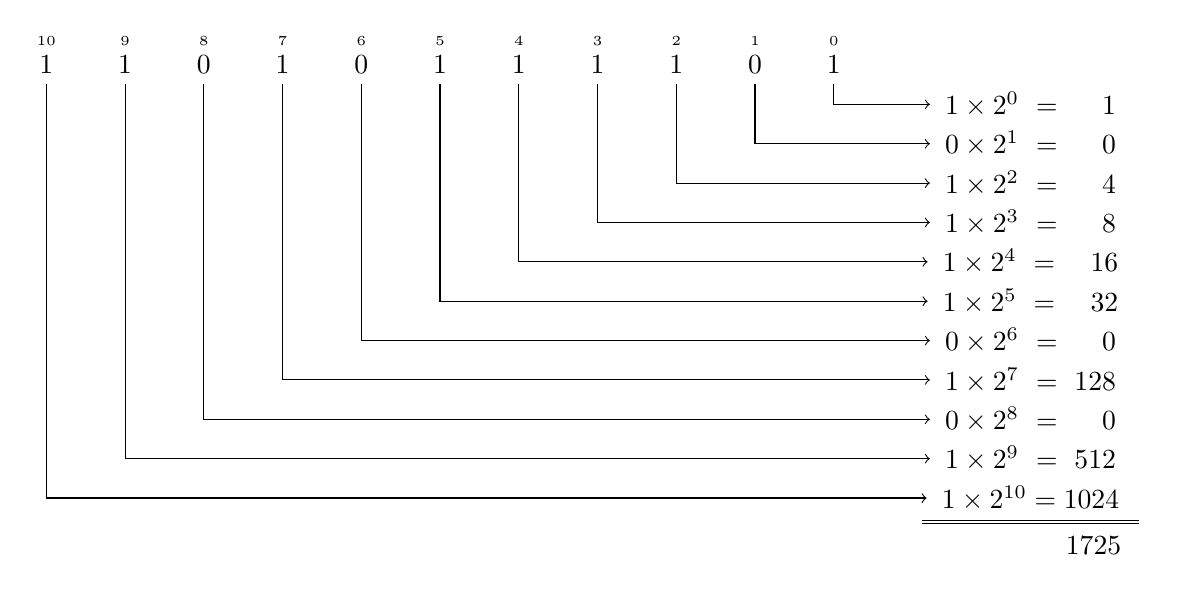
\begin{tikzpicture}[
  flow/.style={draw=black,->,shorten >=2pt}
]
  \node (s10) at (00, 0.8) {\tiny 10};
  \node (s09) at (01, 0.8) {\tiny 9};
  \node (s08) at (02, 0.8) {\tiny 8};
  \node (s07) at (03, 0.8) {\tiny 7};
  \node (s06) at (04, 0.8) {\tiny 6};
  \node (s05) at (05, 0.8) {\tiny 5};
  \node (s04) at (06, 0.8) {\tiny 4};
  \node (s03) at (07, 0.8) {\tiny 3};
  \node (s02) at (08, 0.8) {\tiny 2};
  \node (s01) at (09, 0.8) {\tiny 1};
  \node (s00) at (10, 0.8) {\tiny 0};

  \node (n10) at (00, 0.5) {1};
  \node (n09) at (01, 0.5) {1};
  \node (n08) at (02, 0.5) {0};
  \node (n07) at (03, 0.5) {1};
  \node (n06) at (04, 0.5) {0};
  \node (n05) at (05, 0.5) {1};
  \node (n04) at (06, 0.5) {1};
  \node (n03) at (07, 0.5) {1};
  \node (n02) at (08, 0.5) {1};
  \node (n01) at (09, 0.5) {0};
  \node (n00) at (10, 0.5) {1};

  \node (e00) at (12.5, -0.0) {$1 \times 2^{0} ~= ~~~~1$};
  \node (e01) at (12.5, -0.5) {$0 \times 2^{1} ~= ~~~~0$};
  \node (e02) at (12.5, -1.0) {$1 \times 2^{2} ~= ~~~~4$};
  \node (e03) at (12.5, -1.5) {$1 \times 2^{3} ~= ~~~~8$};
  \node (e04) at (12.5, -2.0) {$1 \times 2^{4} ~= ~~~16$};
  \node (e05) at (12.5, -2.5) {$1 \times 2^{5} ~= ~~~32$};
  \node (e06) at (12.5, -3.0) {$0 \times 2^{6} ~= ~~~~0$};
  \node (e07) at (12.5, -3.5) {$1 \times 2^{7} ~=  ~128$};
  \node (e08) at (12.5, -4.0) {$0 \times 2^{8} ~= ~~~~0$};
  \node (e09) at (12.5, -4.5) {$1 \times 2^{9} ~=  ~512$};
  \node (e10) at (12.5, -5.0) {$1 \times 2^{10} =  1024$};
  
  \draw[flow] (n10.south) |- (e10.west);
  \draw[flow] (n09.south) |- (e09.west);
  \draw[flow] (n08.south) |- (e08.west);
  \draw[flow] (n07.south) |- (e07.west);
  \draw[flow] (n06.south) |- (e06.west);
  \draw[flow] (n05.south) |- (e05.west);
  \draw[flow] (n04.south) |- (e04.west);
  \draw[flow] (n03.south) |- (e03.west);
  \draw[flow] (n02.south) |- (e02.west);
  \draw[flow] (n01.south) |- (e01.west);
  \draw[flow] (n00.south) |- (e00.west);
  
  \node (l0) at (11.0, -5.3) {};
  \node (l1) at (14.0, -5.3) {};
  \draw[double] (l0) -- (l1);
  
  \node (re) at (13.3, -5.6) {$1725$};
\end{tikzpicture}
\end{center}
\captionof{figure}{Decomposition of a binary integer}
\end{defbox}

\emph{Any} positive integer can be transformed in that manner. Note that with $N$ bits, you can form $2^N$ integers, ranging from $0$ to $2^N - 1$.

\subsection{Negative Numbers in Binary}
There are more numbers than positive integers\citationneeded. How do we expand our existing system onto \emph{negative} numbers?

In the world we are used to, there is no problem adding more characters to the set we represent numbers with. In a computer, this would be much more difficult. We somehow have to do with ones and zeros only. A way to solve this is to \emph{limit the number of digits} and select one special digit that is exempt from our interpretation scheme but will serve as a \emph{sign bit}.

\begin{defbox}[Example: Three bit integer with sign bit]
Assume, we use three digits to represent a signed number. Then, the following bitpatterns correspond to these decimal integers:

\begin{center}
\begin{tabular}{cc|cc}
Binary & Decimal & Binary & Decimal \tabcrlf
000 & 0 & 100 & -0 \\
001 & 1 & 101 & -1 \\
010 & 2 & 110 & -2 \\
011 & 3 & 111 & -3
\end{tabular}
\end{center}

The first two bits (bit exponents 0 and 1) are interpreted as before. The \emph{highest order bit} (exponent 2) encodes the sign -- 0 for positive values, 1 for negative ones.
\end{defbox}

While this method fulfils its purpose, it has one glaring weakness: There are \emph{two} representations of the value $0$! This is a problem, since as a human we expect $0 = -0$ to hold; the computer, however, only sees different bitpatterns and therefore declares $0 \neq -0$!

To mitigate this, the so called \emph{two's complement} is employed: the sign bit gets a double role: when computing each digit's contribution, the sign bit is included in the interpretation scheme discussed before, but as a negative value:

\begin{defbox}[Example: Three bit integer with two's complement]
Again, we use three digits to represent a signed number. Then, the following bitpatterns correspond to these decimal integers:

\begin{center}
\begin{tabular}{cc|cc}
Binary & Decimal & Binary & Decimal \tabcrlf
000 & 0 & 100 & -4 \\
001 & 1 & 101 & -3 \\
010 & 2 & 110 & -2 \\
011 & 3 & 111 & -1
\end{tabular}
\end{center}

The first two bits (bit exponents 0 and 1) are interpreted as usual. The \emph{highest order bit} (exponent 2) gives a value of ${\color{blue}-}2^2 = -4$.
\end{defbox}

\begin{warnbox}[Everything is up for interpretation!]
As you see, the same bitbpattern can be interpreted in numerous ways! There is nothing inherent to the sequence of ones and zeros that could tell whether we are dealing with an unsigned or signed integer. As we will later see, this ambiguity also holds for floating point numbers, texts, programs, images, ...

Information in isolation is nigh-worthless. To do anything useful with it, we need some context that provides the way of interpretation for the given information. We will see later on how this is realized in the C programming language.
\end{warnbox}

\subsection{Byte Sized Chunks}
In the human world, we can (in principle) use an arbitrary number of digits to write down any number we fancy. While the binary system does allow the same degree of freedom, computers are more restrictive. Any piece of information will always be composed of an integer multiple of eight bits. We say, information always comes in units of \emph{bytes}.

Several bytes can be joint to form a bigger compound. That is, you can form a (potentially) bigger number out of two bytes. \enquote{Unused} bits will be padded with zeros. For example, the number $15$ could in principle be written as $1111_2$ (in which the index $2$ signifies that this is a binary number.) Since we have to use at least eight bits, in a computer it would be stored as the bitpattern \texttt{00001111}.

\begin{warnbox}[No obvious end]
Again, there is no inherent \enquote{end} of a number. A randomly picked byte from memory could equally well be the start, middle or end of a multi-byte number, or of course a stand-alone one-byte representation of a number. To know which is which, some context is needed which we will have to specify explicitly in our programs.
\end{warnbox}

\section{Binary Representation of Real Numbers}
Real numbers -- numbers with a decimal part, or \enquote{comma values} -- play an important our daily lives. Luckily, computers can handle them as well; of course, this means that there is a way to translate them into binary, as well. The most simple way of doing so would be to specify a fixed position where to insert the decimal point. While this works in principle, it has prooven too inflexible for most real life applications. Instead, a devious scheme to implement \emph{floating point numbers} has been devised. This scheme comes at the cost of introducing a small but sometimes noticeable \emph{rounding error} in each operation that involves such a floating point number.

In this course, we won't be handling floating point numbers a lot; still, it might be interesting for you to better understand how decimal numbers are stored in a binary machine. This is especially helpful when you do scientific simulations and need to minimize rounding errors.

\begin{plusbox}[Representation of real numbers as floating point numbers]
We can follow the same tracks as before when decomposing real numbers: we enumerate all digits of a base ten number, \emph{relative to the position of the decimal point}:
\vspace{\parskip}

\begin{defbox}[Decomposition of a decimal real number]
\begin{center}
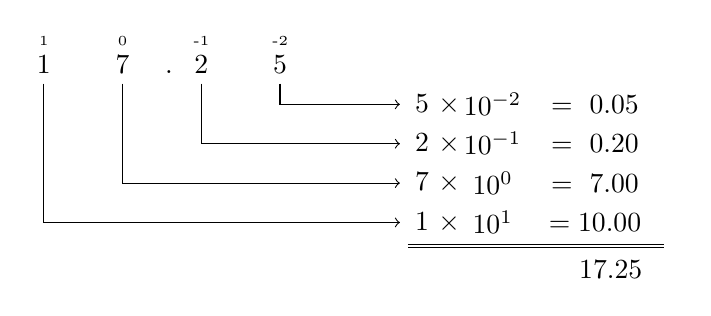
\begin{tikzpicture}[
  flow/.style={draw=black,->,shorten >=2pt}
]
  \node (s3) at (0, 2.3) {\tiny 1};
  \node (s2) at (1, 2.3) {\tiny 0};
  \node (s1) at (2, 2.3) {\tiny -1};
  \node (s0) at (3, 2.3) {\tiny -2};

  \node (n3) at (0, 2) {1};
  \node (n2) at (1, 2) {7};
  \node (nd) at (1.5, 2) {\phantom{0}.};
  \node (n1) at (2, 2) {2};
  \node (n0) at (3, 2) {5};

  \node (e3) at (5.0, 0.0) {$1 ~\times$};
  \node (e2) at (5.0, 0.5) {$7 ~\times$};
  \node (e1) at (5.0, 1.0) {$2 ~\times$};
  \node (e0) at (5.0, 1.5) {$5 ~\times$};
  
  \node (f3) at (5.7, 0.0) {$10^1   $};
  \node (f2) at (5.7, 0.5) {$10^0   $};
  \node (f1) at (5.7, 1.0) {$10^{-1}$};
  \node (f0) at (5.7, 1.5) {$10^{-2}$};
  
  \node (g3) at (7.0, 0.0) {$= 10.00$};
  \node (g2) at (7.0, 0.5) {$= ~7.00$};
  \node (g1) at (7.0, 1.0) {$= ~0.20$};
  \node (g0) at (7.0, 1.5) {$= ~0.05$};

  \draw[flow] (n3.south) |- (e3.west);
  \draw[flow] (n2.south) |- (e2.west);
  \draw[flow] (n1.south) |- (e1.west);
  \draw[flow] (n0.south) |- (e0.west);
  
  \node (l0) at (4.5, -0.3) {};
  \node (l1) at (8.0, -0.3) {};
  \draw[double] (l0) -- (l1);
  
  \node (re) at (7.2, -0.6) {$17.25$};
\end{tikzpicture}
\end{center}
\end{defbox}

The same can be done in binary, again, assuming we have some means of encoding the position of the decimal point (e.g. by fixing the position in the binary representation where it is inserted). Doing so, the decimal number $0.5$ becomes $0.1_2$, the number $0.25$ becomes $0.01_2$ and so forth.

Like in the decimal system, there are numbers that are \enquote{problematic} to write down. Think of the fraction \smallfrac{1}{3} $\approx 0.333...$: you need an infinite number of digits to represent this number in the decimal system. To provide some mathematical insight: this happens whenever in the fractional representation of a number ($\smallfrac{p}{q}$), the denominator has prime factors other than those of ten, \ie other prime factors than 2 and 5.

In the binary system, the base has only one prime factor; hence, such \enquote{problematic} numbers are much more common. As in the decimal system, one simply accepts a little imperfection and works with a rounded number. So, instead of storing the infinite number of digits needed to represent $0.1$ in binary, one simply works with $0.1 \approx 0.0001100110011001101_2$.

You see that a significant number of binary digits is necessary to store the fractional part of a number with acceptable precision. This becomes worse when dealing with very small numbers.

In science, both very small and very large numbers are written down in \emph{scientific notation}: instead of writing $0.025$, one would put $2.5 \times 10^{-2}$ on the paper. This seems tedious for numbers close to 1, but very small numbers like the gravitational constant ($G \approx 6.67430 \times 10^{-11} = 0.0000000000667430$) become \emph{much nicer} to handle this way.

We can do the same in binary: instead of storing the entire information in a singular number, we split it into a \emph{mantissa} ($6.67430$) and an \emph{exponent} part ($-11$) to the benefit of having a way more compact format for our data. Adding a sign bit to the recipe we get a number format that works well for a large range of numbers and uses the available precision as well as possible.

One consequence of this is that larger numbers implicitly are represented with less precision:

Back in the decimal system, think of the mantissa as holding a fixed number of decimal places. Then the uncertainty of this value is given by the exponent. The representation of $2.5 \times 10^{-2}$ could mean anything between $0.0245$ and $0.0254\overline{9}$ -- an uncertainty range of $0.001$. Given the same mantissa but a different exponent, the value $2.5 \times 10^{1}$ covers everything between $24.5$ and $25.4\overline{9}$, an uncertainty range of $1$.

While this rarely causes trouble when \emph{storing} numbers (it is rarely important whether a number is 9289347981238903 or 9289347981238904), problems arise when doing math with numbers of different orders of magnitude.

For example, let's add the numbers $1$ and $0.00001$. Storing them in scientific format with a mantissa lenght of four, they can be represented with perfect precision as $1.000 \times 10^{0}$ and $1.000 \times 10^{-5}$. Let's also assume this is the maximum storage place we want to allot per number. Any number that takes more space than that will be rounded to the next number representable with four mantissa digits. For example, the value $19937$ will be stored as $1.994 \times 10^{4}$.
\end{plusbox}
%
\begin{plusbox}[]
Now, adding $1$ and $0.00001$ together gives $1.00001 = 1.00001 \times 10^{0}$, but would require six mantissa digits -- too much for our limited storage. Hence, the result gets rounded to $1.000 \times 10^{0}$. In other words, we have the \emph{mathematically incorrect} result that $1 + 0.00001 = 1$.

Getting around this problem is non-trivial. Of course, one can always use more mantissa bits (\enquote{more precision}); however, this comes at the cost of higher memory and computation time demand. Designing algorithms with the mechanics behind floating point numbers in mind and thereby minimizing the rounding errors if often the more apt way of dealing with this issue. In this course, we will not focus on this aspect of programming; be aware, though, that it exists.
\end{plusbox}

\section{Binary Representation of Non-Number Information}
Even though the name \emph{computer} already gives away, that these machines are best used for crunching numbers, we also want to (need to) handle information other than pure numbers. To put non-number data into binary memory, again some interpretation scheme has to be applied.

\subsection{Text in Memory}
There are different \emph{encodings} for textual information; all of them are based on the same principle: one can build a one-to-one correspondence between numbers and letters\footnote{or, more general, characters. Technically, \emph{letters} only describes the symbols \emph{a}...\emph{z} and \emph{A}...\emph{Z}, or their counterparts in the various other writing systems. But there's also punctuation, digits and other non-letter constituents of writing systems like line breaks, whitespaces or tabulators.}. We can enumerate all characters of a writing system and use the numbers to stand in for the textual information. For that, we only need to agree on a standard, \ie a ruleset that tells us which character is encoded by which number.

One of the oldest such encoding that is still in use is \emph{ASCII} (American Standard Code for Information Interchange). In ASCII, one byte is used per character, allowing for a theoretical set of 256 different symbols. For technical/historical reasons, only seven of the eight bits are actually in use, limiting the charset to 128 different symbols with their associated number representations. These are depicted in figure \ref{fig:ASCII}.

\begin{figure}
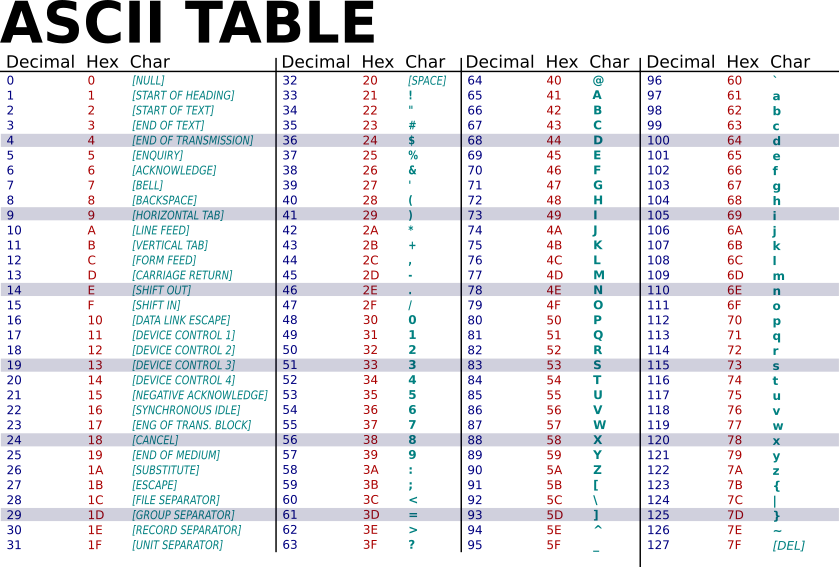
\includegraphics[width=\linewidth]{./gfx/ASCII_table}\newline
\caption
	[ASCII-Codes]
	{ASCII: American Standard Code for Information Interchange\newline
         Source: \url{https://commons.wikimedia.org/wiki/File:ASCII-Table-wide.svg}
    }
\label{fig:ASCII}
\end{figure}

Texts -- \ie strings of letters and other symbols -- are simply sequences of numbers that can be interpreted according to this (or another) table. One nice way of seeing ASCII texts as them being one single number, represented in base 128.

\begin{plusbox}[Other Encodings]
ASCII has been used for a long time, since it can encode most texts with minimal overhead. Especially the \emph{one byte is one character} property means it is easy to work with ASCII text. However, this encoding is rather limiting: there are more than 128 different symbols\citationneeded. Of course it is possible to come up with a longer table and list more characters in it. Essentially, this is the main idea behind Unicode. However, longer tables mean bigger numbers and therefore break the \emph{one byte is one character} property. This also requires some extra thought in order not to waste memory, make texts recoverable even when communication between two machines is flawed or when different communication standards are used.

If you are inclined to learn more, feel free to look up the keyword UTF-8, which is one \emph{encoding system under Unicode}.
\end{plusbox}

\subsection{Graphics and Sound}
A picture can be understood as a collection of pixels in a given order. So a list of pixel data (together with width and height of the complete image) can be used to encode an image. Each pixel is then defined by its colour, which we could again represent by a single number from a table. As there are a lot of colours\citationneeded, it is more convenient to use analogies to the physical world in which these pictures exist to encode the information.

In the case of pictures, we use the fact that humans have photoreceptors for red, green and blue light. Different intensities in these three categories yield the impression of different colours. Hence, storing three numbers per pixel -- one per \enquote{channel} -- is a great way of putting graphical information in memory.

Similarly, sound can be understood as air pressure varied over time. A microphone effectively measures the air pressure over time and reports the current value back to the processing unit (\eg a stero system or a computer). Recording the air pressure every millisecond (and simply ignoring the values in between) is an apt way to store sound information.

\subsection{Computer Programs} \label{sec:assembly}
Much like characters, the various functions a CPU (\emph{central processing unit}) provides are enumerated. There is a command for \emph{load a value from memory into the processor}, another one for \emph{add two values in the processor} and another one for \emph{write a value from the processor buffer into memory}. The very first programmers really had to know (or constantly look up) the numbers of the various commands; their codes were nothing more than long columns of numbers that got fed directly into the processor.

Obviously, this mode of working is rather tedious. A first improvement was to associate each processor command with a short textual representation (a so called \emph{mnemonic}) that is easier to memorize than numbers. A computer program could then \emph{parse} a text file comprising of these mnemonics and translate them into \emph{machine code}. Such a program is called an \emph{assembler}.

While the concept \emph{enumerated commands} holds for all types of CPUs, there is no universal list which number denotes which command. Even worse, different processors have a different \emph{instruction set}, \ie there are different operations that different hardware can execute. Assembly code written for one processor may not be compatible with a different one. There is no \emph{binary compatibility} between different machines. To circumvent this problem, more abstract (and therefore closer to human thinking) languages have been develloped. Code in these languages is \emph{compiled} into assembly code which then can be translated into machine code. Again, this compile step is performed by a dedicated program, the so called \emph{compiler}. The advantage is, that code has to be written only once and can then be deployed on any hardware, for which a compiler exists.

Compiled languages -- like C -- are also more abstract and therefore closer to the way a human thinks. Rather than programming everything on the electronics level, a programmer can focus more on the \enquote{big picture}. Writing code in assembly language is very demanding, the more so if the program has many features and requires large, interconnected code sections. It is very uncommon to write code directly in assembly\footnote{The first generation of the Pokémon gameboy series was written in assembly. While definitely a noteworthy exploit, the many bugs and glitches these games are known for illustrate the difficulty of the feat.}.

I have already hinted at the possibility to load a value from memory into the processor. Of course, for this, the processor needs to know, \emph{which value} to load. You can imagine the memory of a computer as a long row of enumerated cells. Each cell holds exactly one byte of information. Thus, providing the \emph{address}, \ie the number of a memory cell, suffices to provide just that information. In C, we will be dealing with addresses very frequently.

\section{Generating Executable Files} \label{sec:Compile}
With all this theory behind us, we can finally get to practical matters: generating executable programs!

\subsection{Phases of Translation}
You already know that \emph{translating code into machine language} is a fairly complex process. We have talked about \emph{compiling} (translating from a high level language like C into assembly) and \emph{assembling} (translating from assembly language into machine language). Before compilation, theres also a \emph{preprocessing step}, and at the end of the chain of translation phases, theres \emph{linking}.

\emph{Preprocessing} will be discussed in detail in chapter \ref{chp:Preprocessor}. Essentially it is another translation step that allows to write code in a more convenient way. Think of this as a more sophisticated search-and-replace step, that still generates regular C code.

\emph{Linking} means combining multiple files of machine language instructions into a single unit of executable code -- think of it as \emph{glueing together the components of a program}.

\subsection{Invoking the Compiler}
Luckily, all these functions can be executed by a single program (which will invoke other programs to do the four discussed tasks in sequence). This program is the \texttt{gcc}. It combines a preprocessor, compiler, assembler and linker in one program. For convenience, it is usually only referred to as \emph{the compiler}; \emph{to compile} most often means the complete chain of four operations that are needed to generate an executable file.

Naively attempting to start it from the command line will result in an error message:
\begin{cmdbox}[Invoking the compiler without argument]
\$ gcc\\
gcc: {\color{red}fatal error}: no input files\\
compilation terminated.
\end{cmdbox}

That is because, if you want something translated into machine language, you need to tell what this something is. So, assuming we have a file called \texttt{mycode.c} in the current working directory in which there is valid C code, you can tell the gcc that you want to compile that very file by simply passing the filename as a command line argument:
\begin{cmdbox}[Invoking the compiler with argument]
\$ gcc mycode.c
\end{cmdbox}

\begin{warnbox}[Avoid whitespaces in filenames]
You see that whitespaces are what separates the command (\texttt{gcc}) from its arguments (in this case, the file name \texttt{mycode.c}). There can be multiple files that go into one project, and there are also other compiler options which we'll discuss in a minute.

Since all arguments are supposed to be separated by whitespaces, file names with whitespaces are a problem. You can tell the system that a filename contains whitespaces by wrapping the entire name in double quotes:
\begin{cmdbox}[Compiler invocation on a file name with whitespaces]
\$ gcc \textbf{"}my code.\textbf{c"}
\end{cmdbox}

However, it is easier to avoid whitespaces in filenames alltogether.
\end{warnbox}

Provided that the code in \texttt{mycode.c} is syntactically correct (\ie can be translated at all), an output file with the name \texttt{a.out} (under Linux and MacOS) or \texttt{a.exe} will be generated. There will be no output on the console, \ie no error messages (nor success messages). To execute the final result, simply type...
\begin{tcbraster}[raster columns=2,
                  raster equal height,
                  nobeforeafter,
                  raster column skip=0.2cm]
\begin{cmdbox}[Executing a program in Linux/MacOS]
\$ ./a.out
\end{cmdbox}
%
\begin{cmdbox}[Executing a qprogram in Windows]
\$ a
\end{cmdbox}
\end{tcbraster}

If you want to write the compiled output into a different file, you can prepend the command line option \texttt{-o <outputname>}. So for example, to generate a file with the name \texttt{myexecutable}, type:
\begin{cmdbox}[Setting the output filename]
\$ gcc mycode.c \textbf{-o myexecutable}
\end{cmdbox}

\begin{warnbox}[Extensions matter]
I hope you noticed the \texttt{.c} at the end of the code filename. This \emph{filename extension} is not optional. The extension specifies what kind of content can be found in the file. We will soon see that the compiler can process other types of data than C code; to distinguish between how to process different inputs it needs this file extension.

Likewise, the extension of the generated output file should either be \texttt{.exe} if you work on a Windows machine, or none at all on Linux and Mac.
\end{warnbox}

The chain: preprocessing-compiling-assembling-linking can be stopped after the assembly step. The result is a file that contains machine language, but is not directly executable code. This can be useful if some part of the code is used in multiple projects; one can then translate this shared code only once and only do the last step (linkage) with these \emph{precompiled routines}. To do so, one prefixes the command line flag \texttt{-c} to the code file that should be compiled but not linked:
\begin{cmdbox}[Compiling without linking]
\$ gcc \textbf{-c} mycode.c
\end{cmdbox}

After doing so, you will find the file \texttt{mycode.o} on your hard drive. It is called an \emph{object file} and contains the precompiled routines in machine language. Of course, one can combine this with the \texttt{-o} flag to set the output name. For example, \texttt{gcc -c mycode -o myPrecompiledRoutines.o} is a valid command.

These object files can be passed on to the gcc. Since the extension \texttt{.o} marks them clearly as object files, the gcc knows that they only need to parttake in the linkage step. For example, we could run the following two lines:
\begin{cmdbox}[Generating and using object files]
\$ gcc -c sharedRoutines.c -o routines.o \\
\$ gcc mainProject.c \textbf{routines.o} -o projectExecutable
\end{cmdbox}

Some collections of routines are pre-installed on your computer. These collections are called \emph{libraries} and are really only object files packed together. Usually, their filenames begin with the prefix \texttt{lib} and have the extension \texttt{.a}; the name of the library itself is wedged in between. To use these routines in own programs, we can add them add them to the linkage step with the compiler option \texttt{-l<libname>}, where \texttt{<libname>} is the name of the library we want to use. For example, theres the \emph{math library}, which contains routines that help with common mathematical problems such as computing trigonometric functions or finding the square root. This library has the filename \texttt{libm.a}; the \texttt{<libname>} part hence is really only the letter \texttt{m}. It can be added to a project with:
\begin{cmdbox}[Linking against the math library]
\$ gcc myCode.c \textbf{-lm}
\end{cmdbox}
We will use this library frequently in this course.

In the preface I mentioned in passing that the C programming language is still evolving. Over the last fifty years, some features have been added and also some behaviours were changed in a fundamental way. In order to be able to do both, compile old code as it was intended when it was written and use newer features at the same time, the gcc has a \enquote{switch} that allows to select one of several \emph{standards}. For this, we use the command line parameter \texttt{-std=<standard>}, where \texttt{<standard>} specifies which version of the language should be expected. In this course, we'll be using the Standard from 2017, which goes by the code \texttt{c17}. So, our invocations of the compiler will need the according option set every time:
end um \texttt{-std=c11}:
\begin{cmdbox}[Compiling with the language standard from 2017]
\$ gcc \textbf{-std=c17} myCode.c
\end{cmdbox}

As humans, we are prone to making errors. \emph{Very} prone. I started programming as a hobby more than twenty years ago, and still I hardly write more than some ten lines of code before I check whether I've made any mistake. And there are many mistakes one can make. Some simply render a program \enquote{nonsensical}, \ie prevent translation into machine language alltogether. Others are more subtle; they are valid instructions, but have unintended side effects. The gcc is actually capable of detecting some patterns in code files that were most likely not intended by the programmer. If such patterns are detected, a \emph{warning} is printed on the console -- at least if enabled by the appropriate command line options. Since there are different \enquote{levels of warnings}, there are multiple options: \texttt{-Wall} enables \emph{all} basic warnings; \texttt{-Wextra} adds some more warnings, and \texttt{-Wpedantic} requires the programmer to adhere to a very strict ruleset.

Maybe you're much smarter than I am and don't need this sort of assistance; I for one have been very happy about these features. More often than not they prevented bugs or made me aware of problematic constructs. Therefore, I highly recommend you to compile your codes with these three options:
\begin{cmdbox}[Enabling useful warnings]
\$ gcc \textbf{-Wall -Wextra -Wpedantic} myCode.c
\end{cmdbox}

Since all of this is quite a mouthful to retain, you can look up all of these and other options in the appendix. See table \ref{tab:CompilerOptions} at the end of this book.

To put it in a nutshell, when writing code I recommend you to type these commands; they will soon enough become a second nature:
\begin{cmdbox}[My standard compiler invocation]
\$ gcc -std=c17 -Wall -Wextra -Wpedantic myCode.c -lm -o executable \\
\$ ./executable
\end{cmdbox}

\section{Main Takeaways} 
\begin{itembox}[Binary Data]
\item All information is stored as bitpatterns that have no inherent meaning. What a given sequence of bits means depends on which interpretation rules are applied
\item All information is grouped in bytes, \ie groups of eight bits. Multiple bytes can be compounded to form a larger piece of information.
\item There is a principal difference between integers and floating point numbers.
\end{itembox}
%
\begin{itembox}[Translating Code]
\item C code is translated into executable files in four steps: preprocessing, compiling, assembly and linkage. The gcc can do all these steps in one go.
\item C code files need to have the extension \texttt{.c}.
\item C code can be compiled once into object files and used in several projects. Object files have the extension \texttt{.o}
\item Libraries are collections of object files that can parttake in the linkage process. To do so, use the option \texttt{-l<library name>}
\item Depending on the operating system, executable files should either have no extension (Linux, Mac) or the extension \texttt{.exe}
\item To set an output name, use the option \texttt{-o <output filename>}
\item There are different language standards for the C programming language. A standard can be selected with the option \texttt{-std=<standard>}. We use \texttt{-std=c17} in this course.
\item The compiler can analyze the code for suspicious lines that most likely generate undesired behaviour. To enable this feature, add the compiler options \texttt{-Wall -Wextra -Wpedantic}.
\item For most of our projects, the compiler invocation should look like this:\\
	\texttt{gcc -std=c17 -Wall -Wextra -Wpedantic myCode.c -lm -o executable}
\end{itembox}

\newpage
\section{Exercises and Solutions}
\subsection*{Translating Binary}
\begin{itemize}
\item Which positive integer corresponds to the bit sequence $101010_2$?
\item Which bit sequence corresponds to the decimal number $21_{10}$?
\item Which bit sequence corresponds to the string \texttt{42}?
\end{itemize}

\subsection*{Pitfalls in binary encoding}
\begin{itemize}
\item Why does it matter for a computer whether a number is given as $2.0$ or as $2$?
\item You are given a sequence of 16 bits together with the information that they encode an unsigned integer. Why is even this information not enough to unambiguosly decode the bit sequence?
\end{itemize}

\subsection*{Phases of Translation}
Recapitulate on the translation phases: What happens in which order when we invoke the gcc?

\rule{\linewidth}{0.1mm}

\subsection*{Solution: Translating Binary}
\begin{itemize}
\item $101010_2 = 42_{10}$
\item $21_{10} = 10101_2$. \\
	Notice how $42 = 2 \times 21$ and how, in binary, you get from $21$ to $42$ by adding a zero.\\
	Do you see how this is related to the fact that $2_{10} = 10_2$?\\
	(Multiplying with ten in the decimal system also only adds a zero to the number representation)
\item The \emph{string} \texttt{42} comprises of two \emph{characters}, \texttt{4} and \texttt{2}.\\
	From the ASCII table (fig. \ref{fig:ASCII}) we find that \texttt{4} has codepoint 52 and \texttt{2} has codepoint 50.\\
	Converting these codepoints into binary gives the bit sequence \texttt{0011 0100  0011 0010}.
\end{itemize}

\subsection*{Solution: Pitfalls in binary encoding}
\begin{itemize}
\item Albeit mathematically equivalent, $2.0$ is a \emph{floating point number} and will thus be encoded in a different manner than the \emph{integer} $2$.
	This means the form of the bitpattern and possibly also the number of bytes required to store the information will be different.
\item 16 bits are 2 bytes; these two bytes can be read from the left to the right or the other way round. One also has to specify a \emph{byte order}.\\
	The byte order is hard wired into the machine, so this won't have any impact on what we do in this course; however, when communicating with other machines,
	one has to keep in mind that the other machine might use a different byte order.´
\end{itemize}

\subsection*{Solution: Phases of Translation}
A C code file undergoes these phases of translation:
\begin{description}
\item[Preprocessing] \hfill \\
	Replaces parts of the input file with other lines of C-Code.
\item[Compiling]     \hfill \\
	Translates the (mostly machine-independent) in (machine dependent) assembly language, produces assembly files
\item[Assembly]      \hfill \\
	Translates assembly language code into machine language, produces object files
\item[Linkage]       \hfill \\
	Gathers object files and libraries and puts them together in one single executable
\end{description}